\section{\normalsize  Среднее число молекул, сталкивающихся в единицу времени с единичной площадкой. Средняя энергия молекул, вылетающих в вакуум через малое отверстие.}
\paragraph{ Среднее число молекул, сталкивающихся в единицу времени с единичной площадкой.} 


\begin{wrapfigure}{L}{5cm}
	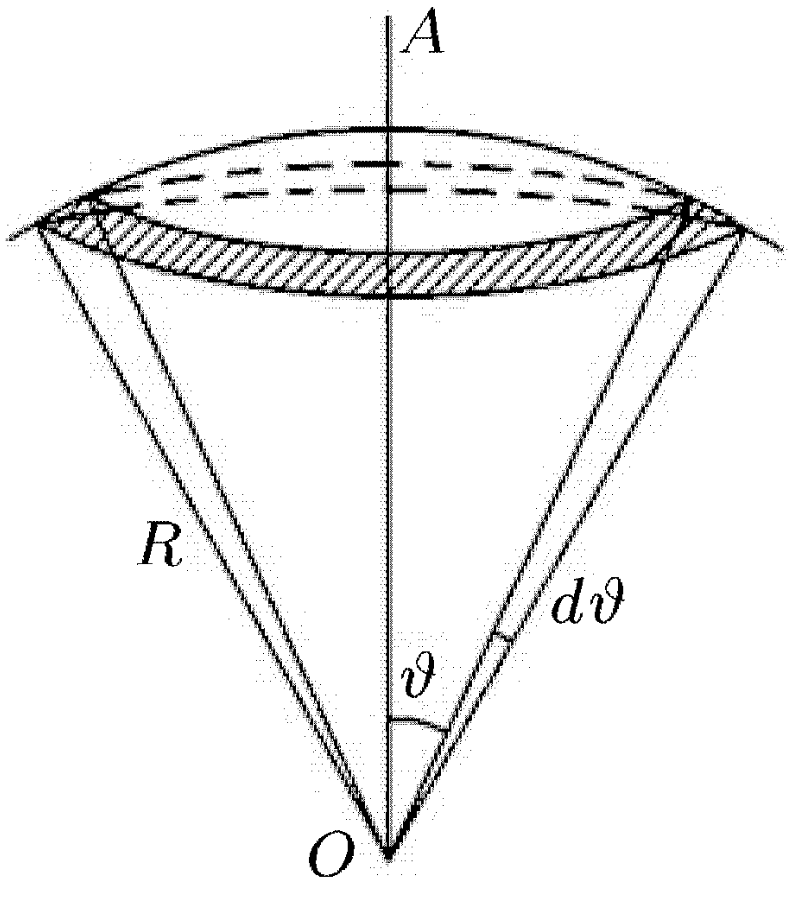
\includegraphics[width=50mm]{ris27.png}
\end{wrapfigure}$\;$\\
$\Omega = 2\pi(1-\cos\vartheta);\ d\Omega=2\pi\sin\vartheta\, d\vartheta;\\ dN=N\frac{d\Omega}{4\pi}=\frac{N}{2}\sin\vartheta\, d\vartheta$ --- среднее число молекул, направления скоростей которых лежат в пределах телесного угла $\Omega$ и образующие углы между $\vartheta$ и $\vartheta+d\vartheta$ с направление OA.\\
Выделим группу молекул с x-компонентами скоростей от $v_x$ до $v_x+dv_x$, $v_x>0$. Пусть их число в единице объема $dn_\vartheta$, тогда число их ударов о 1см$^2$ за 1с: $d\nu_\vartheta=dn_\vartheta v_x=\\=0.5n \sin \vartheta\cos\vartheta\,d\vartheta\,v$
\[d\nu_{\vartheta, v} =\frac{n}{2}\sin\vartheta\cos\vartheta d\vartheta v F(v)dv=\]\[=\frac{n}{2}\sin\vartheta\cos\vartheta d\vartheta v 4\pi v^2\left(\frac{m}{2\pi kT}\right)^{3/2}\exp\left(-\frac{mv^2}{2kT}\right)=\]\[=2\pi n\left(\frac{m}{2\pi kT}\right)^{3/2}\left[v^3 \exp\left(-\frac{mv^2}{2\pi kT}\right)dv\right]\left[sin \vartheta\cos\vartheta d\vartheta\right]\Rightarrow\]\[\Rightarrow \nu=2\pi n\left(\frac{m}{2\pi kT}\right)^{3/2}\int_{0}^{\infty}v^3\exp\left(-\frac{mv^2}{2kT}\right)dv\int_{0}^{\pi/2}\sin\vartheta\cos\vartheta d\vartheta=\frac{n\overline{v}}{4}   \]
\paragraph{ Средняя энергия молекул, вылетающих в вакуум через малое отверстие.} Будем рассматривать одноатомный газ. $dn$ --- число молекул в 1 см$^3$, обладающих скоростью в интервале $(v,v+dv)\Rightarrow dn=nF(v)dv$.\\
За 1 секунду из отверстия вылетает $1/4dn\,v$, которые унесут $\frac{mv^2}{2}1/4dn\,v\Rightarrow$
\[ \Rightarrow E_\text{полн.}=\int1/4\frac{mv^2}{2}dn\,v=\int_{0}^{\infty}\frac{m}{8}v^3nF(v)dv\Rightarrow \overline{E_\text{выл.}}=\frac{E_\text{полн.}}{\int_{0}^{\infty}1/4nvF(V)dv}=\]\[=\frac{m/2\int_{0}^{\infty}v^5e^{-\lambda v^2}dv}{\int_{0}^{\infty}v^3e^{-\lambda v^2dv}}=\frac{m}{\lambda}=2kT   \]